\documentclass[
%draft,
11pt,
titlepage,
reqno,
%	oneside,
%	twocolumn
]{article}%Draft option puts "slugs" in the margin for overfull lines

%\usepackage{newlattice}%custom package by Gratzer. Use with amsart See book for details.
%Packages loaded by amsart:
%\usepackage{amsmath}%This loads amsbsy, amsopn, amstext
%\usepackage{amsfonts}
\usepackage{amsthm}%This loads amsgen
\usepackage{amsxtra}
\usepackage{geometry}

%\usepackage{pdfsync}
%\usepackage{upref}
%\usepackage{amsidx}
%\usepackage{stmaryrd} %This adds small left arrows for accents that more closely mirror the \vec command
\usepackage{amssymb}
\usepackage{mathtools}
\usepackage{latexsym}
\usepackage{amsmath}
\usepackage{natbib}
\usepackage{exscale}
\usepackage{amscd} %commutative diagrams
\usepackage{dcolumn} %to get decimal places aligned in tables
\usepackage{array}
\usepackage{tabularx}
%\usepackage{MnSymbol} %dashed arrows and more - see documentation
\usepackage[mathscr]{eucal}
\usepackage[english]{babel}
\usepackage[pdftex]{graphicx}
\usepackage{subcaption}%for tables and such
\usepackage{lipsum} %for preventing breaks and such
%\usepackage{pgf,pgfarrows,pgfnodes,pgfshade}
\usepackage{setspace} %Turn ON for editing
%\usepackage{verbatim}
%\usepackage{enumerate}
%\usepackage{xspace}`
%\usepackage{longtable}
%\usepackage{epstopdf}
%\usepackage[authoryear]{natbib}
%\usepackage{lscape}


%\theoremstyle{plain}
\newtheorem{acknowledgement}{Acknowledgement}
\newtheorem{assumption}{Assumption}
\newtheorem{axiom}{Axiom}
\newtheorem{case}{Case}
\newtheorem{claim}{Claim}
\newtheorem{conclusion}{Conclusion}
\newtheorem{condition}{Condition}
\newtheorem{conjecture}{Conjecture}
\newtheorem{corollary}{Corollary}
\newtheorem{criterion}{Criterion}
\theoremstyle{definition}
\newtheorem{definition}{Definition}
\newtheorem{econjecture}{Empirical Conjecture}
\newtheorem{example}{Example}
\newtheorem{exercise}{Exercise}
\newtheorem{lemma}{Lemma}
%\theoremstyle{remark}
\newtheorem{remark}{Remark}
\newtheorem*{notation}{Notation}
\newtheorem{proposition}{Proposition}
\newtheorem{theorem}{Theorem}
\newtheorem*{main}{Main Theorem}
\newtheorem{solution}{Solution}
\newtheorem{summary}{Summary}
%\newenvironment{proof}[1][Proof]{\noindent\textbf{#1.} }{\ \rule{0.5em}{0.5em}}

\newcommand{\BigFig}[1]{\parbox{12pt}{\Huge #1}}%See Gratzer l. 2442 (for matrix)
\newcommand{\BigZero}{\BigFig{0}}

\doublespacing %This is a command from the SetSpace package

\geometry{letterpaper}
\setlength{\oddsidemargin}{0in}
\setlength{\topmargin}{0in}
\setlength{\topskip}{0in}
\setlength{\headsep}{0in}
\setlength{\headheight}{0in}
\setlength{\textwidth}{6.5in}
\setlength{\textheight}{8.75in}

%junk comment for Git

\begin{document}
	
	\title{Notes on Group! Agency\thanks{}
	}
	\author
	{
		Brian Epstein \\Tufts University, Medford
		\and 
		Michael D.\ Ryall \\University of Toronto 
	}
	\date{\today}
	\maketitle
	
	%\begin{abstract}
	
	%\end{abstract}
	
	%\doublespacing
	\def\baselinestretch{1.5}\small\normalsize
	
	\newpage
	\section{Overview}

	This version begins with a model of individual agency in Section \ref{sec:individuals}, then moves on to groups and group agency in the remaining sections. 
	We are aiming for a  formal framework that is fairly general, thereby allowing for a substantial degree of flexibility in the sorts of phenomena it can represent.  
	The formalism for groups builds on the individual setup. 
	
	\section{Notational conventions}
	\subsubsection{General}
	Capital letters ($G$, $N$, etc.) refer to sets.  
	Small Arabic and Greek letters refer variously to elements of sets (e.g., $i\in N$) and functions (e.g., $\sigma:N\rightarrow \mathcal{N}$). 
	Terms  are \textit{italicized} at the point of definition.  
	A \textit{profile} is a placeholder for a list of elements.
	We denote these in boldface: e.g., $\mathbf{x}$ where $\mathbf{x}\equiv(x_1,\ldots,x_n)$. 
	The ``$\equiv$'' symbol indicates the definition of a mathematical object. 
	If $X$ is a set, then $2^X$ is the notation denoting the set of all subsets of $X$. Calligraphic letters refer to sets of sets (e.g. $\mathcal{X}\equiv 2^X$). 
	Curly parentheses indicate sets, typically in defining them (e.g. $X\equiv\{x|x\text{ is an even integer}\}$). 
	The notation ``$|\cdot|$'' indicates set cardinality (e.g., if $X\equiv\{a,b,c\}$, then $|X|=3$). 
	If $X$ is a set and $Y\subset X$, then $X\setminus Y$ is the set $X$ minus $Y$; i.e., the set of elements of $X$ that  remain when the elements of $Y$ are removed. 
	All sets are assumed to be finite unless otherwise indicated.

	\subsubsection{Specific}
	The following table elaborates all the mathematical objects used in the paper.

	
	
	
	\section{Individual Agency}\label{sec:individuals}

	Begin with a \textit{population of individuals}, indexed by the set $N\equiv \{0,\ldots,n\}$ with typical element $i\in N$ and $\mathcal{N}\equiv 2^N$. For now, we focus on an individual actor. 
	Later, we consider groups. The evolution of the world through time is driven by the actions of individuals as well as of the onset of natural phenomena. 
	We account for natural phenomena as the ``actions'' of  Nature which we assign to population index 0.

	We break this section into two subsections. The first develops the mathematical machinery to discuss and analyze actual and  potential states of the world at a moment in time. We refer to this as the \textit{synchronic} perspective.  With these details in place, we then extend the framework to the dynamic case, in which the world evolves through time. We refer to this as the \textit{diachronic} perspective.  
	
	
	\subsection{Synchronic Setup}\label{sec:synchronic_setup}

	\subsubsection{States\label{sec:states}}

	A \textit{state}, denoted $s$, is a snapshot of the world at a moment in time.
	States elaborate the status \textit{of all features of the world} in that moment. 
	This includes the relevant ``mind-independent'' features of a particular world as well as the ``mind-dependent'' features of the individuals acting in that world. 
	Clearly, it would require an uncountably infinite number of states to elaborate everything about the world in a given moment, much less all the potential features that could be actualized in that moment.
	However, our discussion will always focus upon a finite set of actors who are typically concerned with a particular set of issues.
	Therefore, we sidestep some mathematical complexities by limiting our attention to the relevant features by assuming that the potential number of states required to describe the features of interest at any particular moment are finite.

	With this in mind, let $S^0$ denote the (finite) set of all possible states of the world.
	The  ``0'' superscript indicates that this corresponds to Nature's ``perception'' of reality; i.e., $s\in S^0$ is a description of the real world as it could actually exist. 
	Individual superscripts, e.g., $S^i$, $i\ne 0$,  indicate individual $i$'s (typically, limited) awareness of reality.
	Specifically, we assume $\mathcal{S}\equiv \{S^\emptyset,S^0,S^1,\ldots,S^n\}$ along with $\succeq$, a partial order on $\mathcal{S}$, is a complete lattice in which $S^0$ is a maximum (the richest expression of reality) and $S^\emptyset$ is a minimum (the poorest expression), where $S^\emptyset\equiv\{\emptyset\}$ is defined as the state space consisting of a single element (i.e., in which nothing about the world is distinguished).\footnote
	{
		Here, we adapt the interactive unawareness approach developed by \cite{Heifetz2006
		}
	}
	Let $\Sigma\equiv\bigcup_{i\in N}S^i$ denote the union of the individual spaces.
	
	Conceptually, for an actual individual $i$, $s^i\in S^i$ includes all the features of reality that individual $i$ can bring to mind and relate to in the moment at hand.
	Thus, $S^i\succeq S^j$ means that individual $i$ is able to distinguish at least as much about the world as individual $j$ in that moment.
	Because $\succeq$ is a partial order, not all state spaces are comparable; i.e., individuals $i$ and $j$ may be aware of different things in a given moment.

	We wish to keep track of how the different state spaces relate to reality ($S^0$) and, when possible, to each other. 
	Therefore, define the surjective \textit{projection} $r^{i\rightarrow j}:S^i\rightarrow S^j$, which is only defined if  $S^i\succeq S^j$.
	Then, $s^j=r^{i\rightarrow j}(s^i)$ is the impoverished version of reality $j$ perceives relative to the awareness of $i$. 
	By assumption, for all $i\ne 0$, $S^0\succeq S^i$.
	Assume the projections are commutative: if $S^i\succeq S^j\succeq S^k$, then $r^{i\rightarrow k}=r^{j\rightarrow k}\circ r^{i\rightarrow j}$.
	
\begin{figure}[h!]	
	\begin{center}
		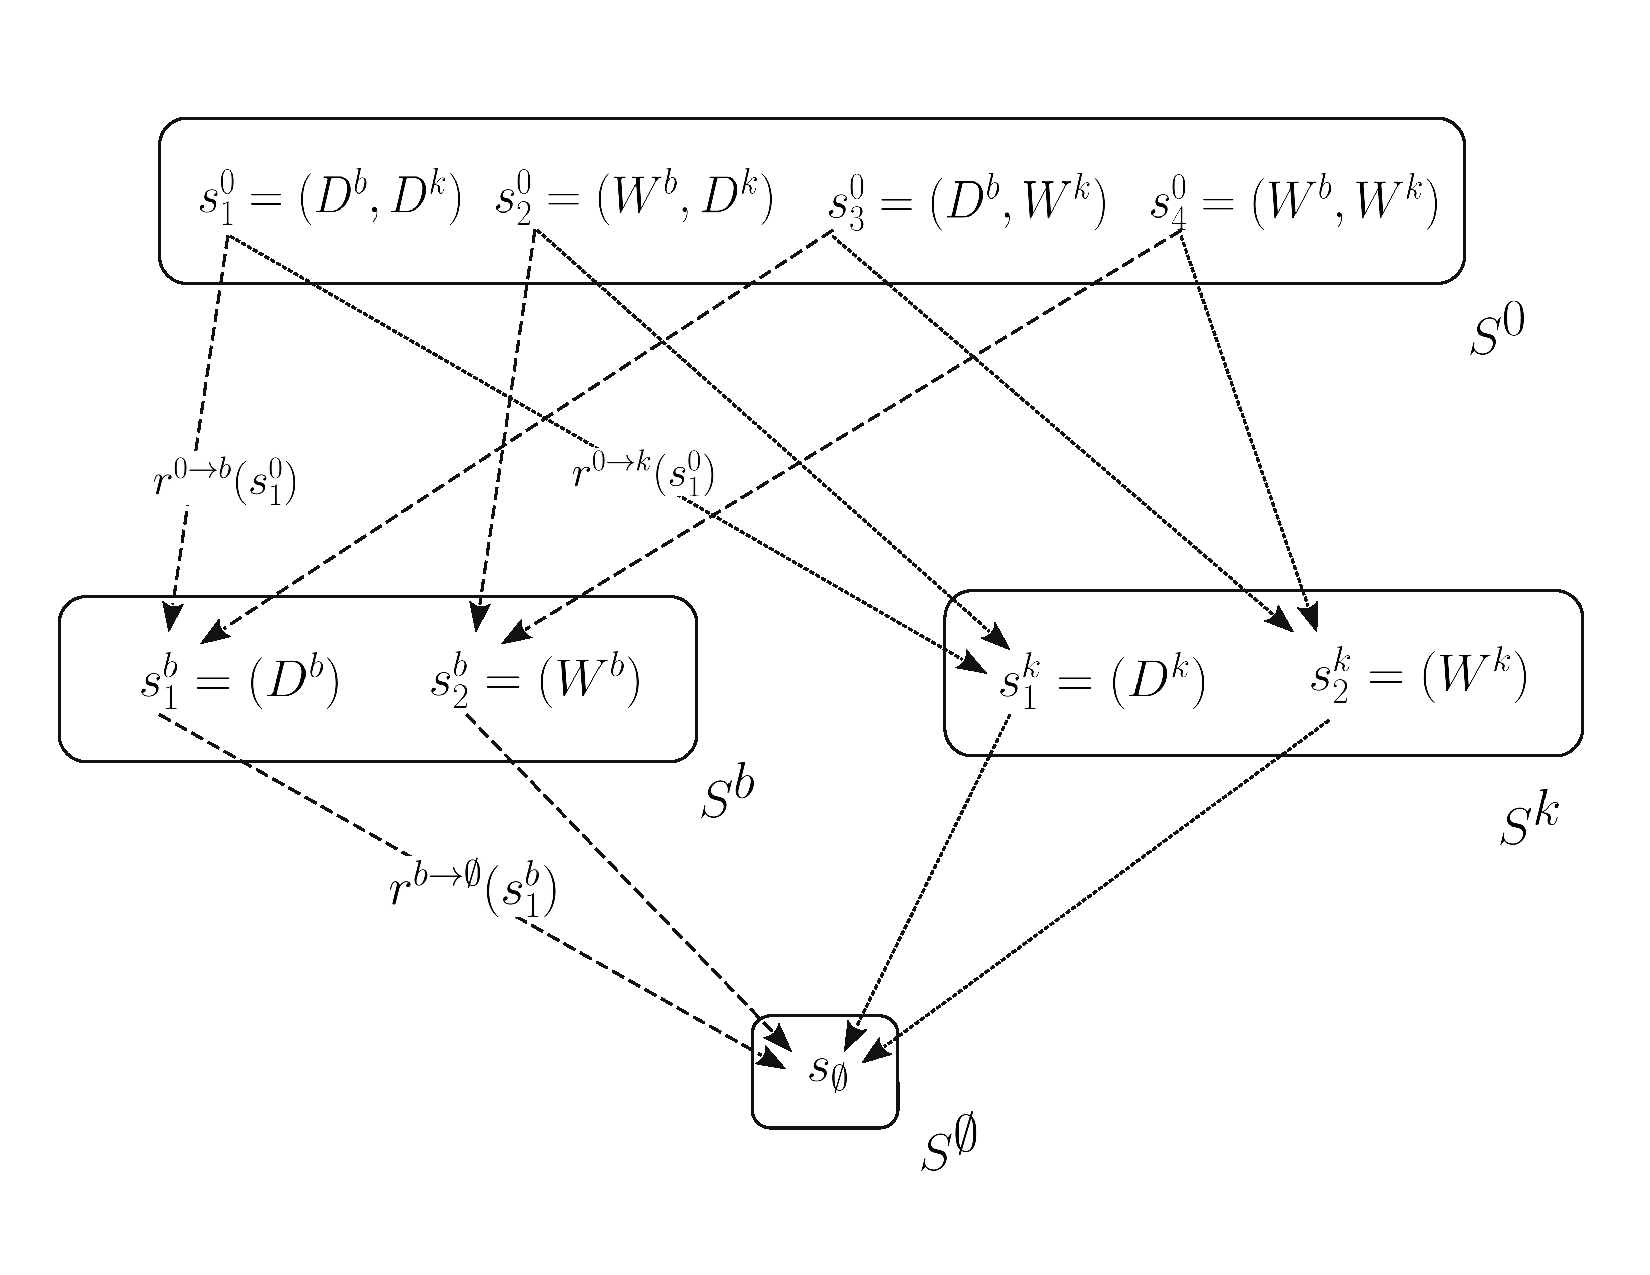
\includegraphics[scale=.7]{lattice.png}
	\end{center}
\caption{Awareness of Irene and Ken\label{lattice}}
\end{figure}

	To see a simple example of the setup, consider a situation in which  Irene ($i$) and Ken ($k$) form an intention of whether or not to take a walk together. 
	Let $I_i$ and $\neg I_i$ indicate that Irene intends or does not intend, respectively, to take a walk with Ken and, similarly, for Ken. 
	Then, in this simple world, there are four states that can be true: $(I_i,I_k),(I_i,\neg I_k),(\neg I_i,I_k)$ and $(\neg I_i,\neg I_k)$. 
	In Figure \ref{lattice}, we see the individual spaces represent a world in which Irene and Ken are only aware of their own intentions. 
	The projections are shown as dashed lines, with $r^{0\rightarrow i}(I_i,I_k)$ and $r^{i\rightarrow \emptyset}(I_i)$ specifically labelled. 
	Thus, if $(I_i,I_k)$ is the true state of the world, then Irene is only aware of her intention and, similarly, Ken is only aware of his intention. 
	As required, the figure includes the state of complete unawareness, $S_\emptyset$.
	Note that, while $S^0_t\succeq S^i_t\succeq S_\emptyset$ and $S^0_t\succeq S^k_t\succeq S_\emptyset$, $S^i_t$ and $S^k_t$ are neither richer nor poorer than the other.
	Here, $\Sigma$ is the set containing all the states from all the state spaces.

	\subsubsection{Synchronic events}

	The term `event' is used differently in philosophy than it is in probability theory. 
	Since we are writing to audiences familiar with one or the other, it is important to clarify this difference. 
	In probability theory, `event' is used similarly to the term `property' in philosophy, where properties are understood intensionally. 
	Philosophers typically use `event' to mean a spatiotemporal particular extended over time. 
	We refer to events associated with states at a moment in time (the game theory useage) as \textit{synchronic events}, and those associated with states unfolding through time (the philosophy usage) as \textit{diachronic events}.
	Below, we define the former.
	We wait to define the latter until Section \ref{sec:diachronic_setup}.
	
	In probability theory, events are subsets of state spaces. 
	For example, the event ``Mike intends to get a cup of coffee includes \textit{all} states in which getting a cup of coffee is the intention of Mike. 
	In philosophical terminology, this is equivalent to the property \textit{being in a state in which Mike intends to get a cup of coffee,} where the intension of the property is all the states of the world in which the world exemplifies that property.
	Because each individual is associated with a state space that elaborates states according to the features of the world of which that individual could be aware in a given moment, the events of which he or she could be aware are subsets of that space. 
	For example, $E=\{s\in S^i|s\Rightarrow \text{Mike has coffee}\}$ is the event, which $i$ is aware of as a possibility, that Mike has a cup of coffee (i.e., all the states in which this obtains according to $i$).

	Because individual state spaces may be related to one another and, in any case, are all related to reality fully elaborated ($S^0$), it will be helpful to consider the events that can be described in one individual space to those implied in spaces that are at least equally as rich.
	To set this up, let $g:\mathcal{S}\rightarrow 2^{\mathcal{S}}$ where $g(S^j)\equiv\{S^i\in\mathcal {S}|S^i\succeq S^j\}$ identifies the set of state spaces that are at least as rich as $S^j$.
	For a state-space event $B\subseteq S^j$, let $B^{\uparrow}=\bigcup_{S^i\in g(S^j)}\left(r^{i\rightarrow j}\right)^{-1}(B)$ be the extension of $B$ to include all states in other individuals' state spaces that provide elaborations of reality that are at least as rich as $S^j$.
	Then, $E\subseteq \Sigma$ is a \textit{synchronic event} if it is of the form $B^{\uparrow}$ for some $B\subseteq S^i\in \mathcal{S}$.
	We refer to the state space event, $B$, as the \textit{basis} of the extended event $E=B^{\uparrow}$ and to $S^j$ as the \textit{base-space} of $E$.
	By this definition, not every subset of $\Sigma$ is a synchronic event.
	If $B\subseteq S^j$, define the negation of the synchronic event $B^{\uparrow}$, denoted $\lnot B^{\uparrow}$, as $(S^j\setminus B)^{\uparrow}$, typically a proper subset of $\Sigma\setminus B^{\uparrow}$.

	\begin{figure}[h!]	
		\begin{center}
			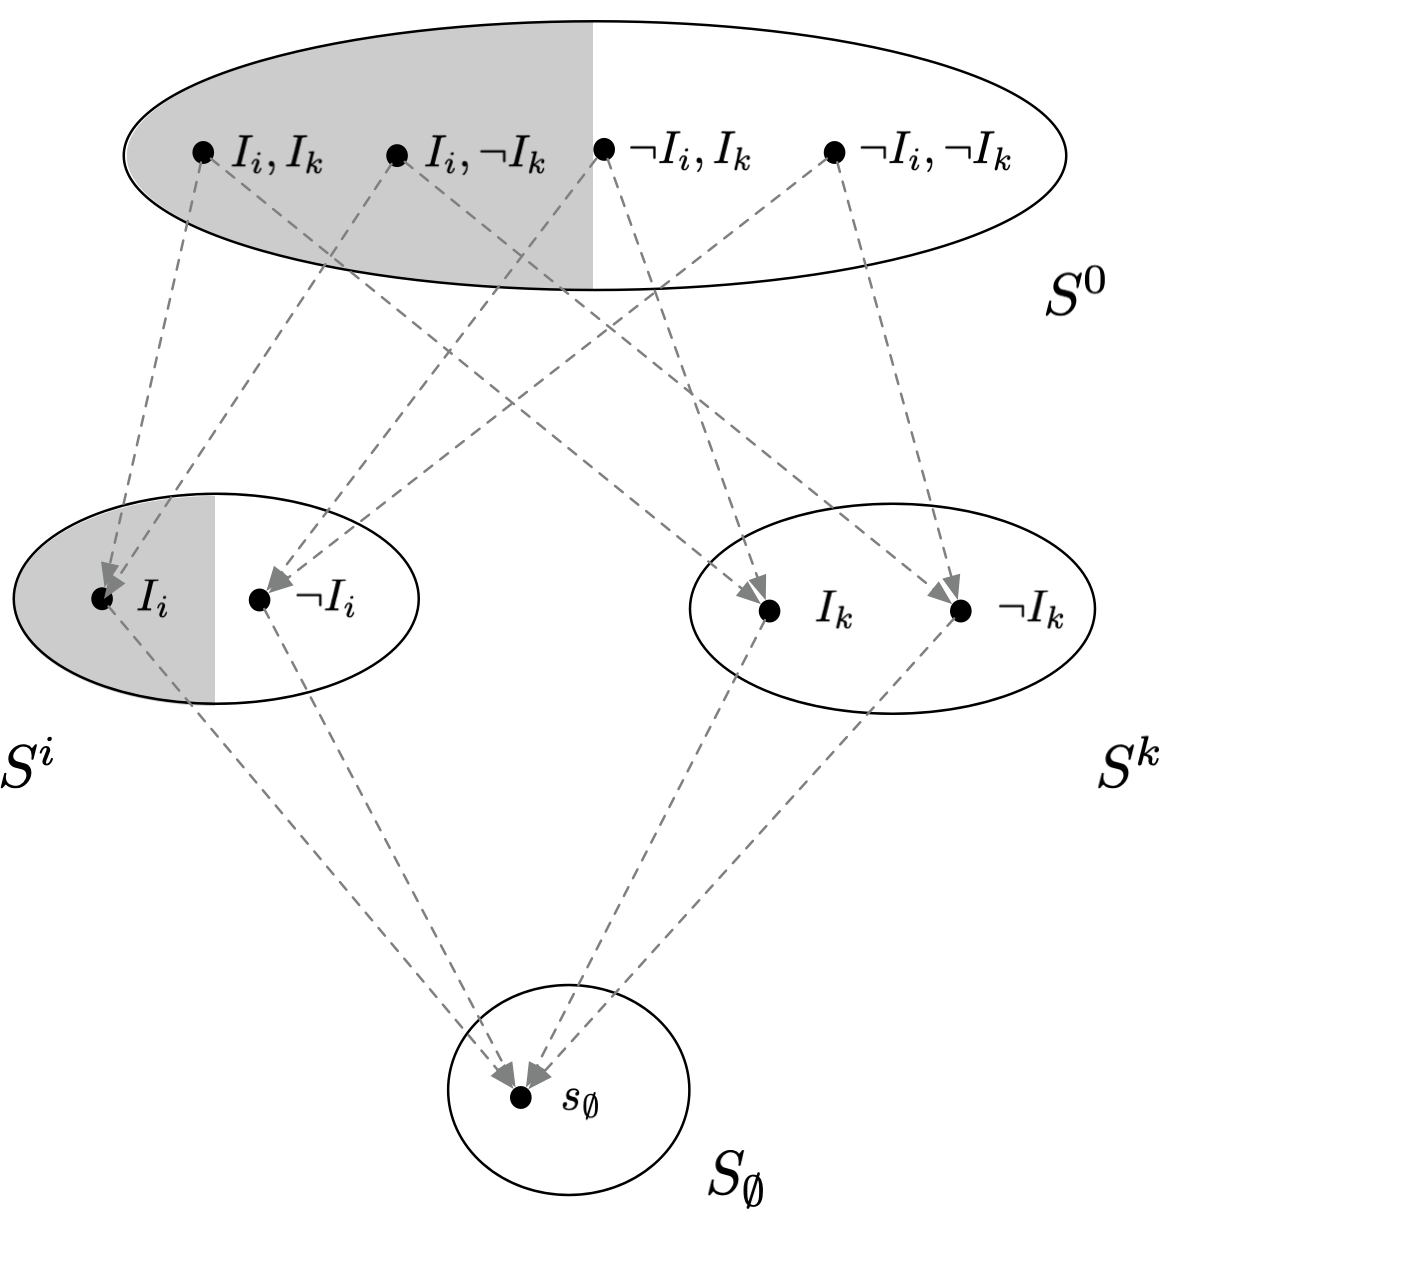
\includegraphics[scale=.7]{lattice-event.png}
		\end{center}
		\caption{The awareness structure event ``Irene intends to walk with Ken''\label{lattice-event}}
	\end{figure}
	
	 Returning to our example with Irene and Ken, consider the event ``Irene intends to take a walk with Ken'' in $S^i$. 
	 Let $B=\{I_i\}\subseteq S^i$ be this state-space event.
	 Then, $B$ is the basis of $B^{\uparrow}=\{(I_i,I_k),(I_i,\lnot I_k),I_i\}$ and $S^i$ is the base-space.
	 Notice that $\lnot B^{\uparrow}=\{(\lnot I_i,I_k),(\lnot I_i,\lnot I_k),\lnot I_i\}$.
	 Thus, $B^{\uparrow}\cup \lnot B^{\uparrow}$ is a strict subset of $\Sigma$.
	 We also see that the states in an individual state space represent a coarsening of reality (formally, a partition of $S^0$) due to the fact that the projections are surjective functions from more refined spaces to coarser spaces.

	 +++++++++++++++++++++++++++++++++++STOPPED HERE++++++++++++++++++++++
	
	\subsubsection{Mental attitudes\label{sec:attitudes}}
	In what follows, we develop an awareness-belief-desire-intention model of mental attitudes. 
	The essential aim of this formalism is to take seriously the cognitive constraints we face as finite, material beings.
	In particular, we proceed from the uncontroversial claim that, at any given moment, an individual can only  attend to some finite number of conscious concerns. 
	We say that an individual is \textit{aware} of the matters toward which his or her attention is directed.
	Under constrained awareness, intentions take on an important role that is distinct from beliefs and desires.
	
	The idea is as follows.
	To the extent some share of the mind's resources are occupied in solving a problem (e.g., deciding what kind of car to buy), those resources are not available for other conscious operations, such as solving other problems, constructing a feasible plan by which to acquire a car, or actualizing that plan by driving to the car dealer and making the transaction.
	We conjecture that an individual's finite stock of cognitive resources almost always acts as a hard constraint on his or her decision- and act-making capability.
	In our model, intentions serve as the pivot from goal assessment to goal acquisition.
	The formation of an intention moves an individual from a state in which an individual is reckoning what to do to a new state in which the individual has decided what to do and in which he or she has at least some sense of how to proceed -- i.e., a \textit{plan}.\footnote
	{
		A more elaborate treatment might well separate each step by an act of intention: first, the move from goal assessment to plan selection; then, from plan selection to plan implementation. For now, we bundle these steps into one.
	}
	Thus, forming an intention frees up the mental resources required to determine which goal to pursue and how to pursue it.
	When events arise consistent with the plan, the individual can act accordingly -- without engaging the mental machinery required to reassess goals and plans.
	Because deciding to focus attention on some new problem can, itself, be an intentional goal, one's awareness is dynamic and, to some extent, influenced by one's own intentions.
	As we will see, there are also social implications as individuals become aware of the intentions of others.  

	Beliefs and desires will operate in a familiar way. 
	The distinction here is that they are restricted to those matters about which an individual is aware.
	As we show below, because beliefs cannot account for awareness and because intentions shift awareness, a belief-desire model cannot do the work of an awareness-belief-desire-intention model.



	% As we elaborate below, we assume that the status of one's mental attitudes at time $t$ is a feature of the actualized state $s_t$. 
	% First, we define \textit{beliefs} as subjective conjectures about the likelihood of past events, the present state, and future events. 
	% Second, \textit{desires} are the individual's attitudes toward histories, represented as a partial order relation on $\mathcal{H}_T$. 
	% In other words, individuals consider both the sequences of states they experience as well as the acts that induce them.
	% For example, even though a junior faculty member may have the same degree of desire for tenure at her present institution in all states of the world in which that happens, some paths to tenure may be more costly than others depending upon the acts required to get there (both her own and others, including those by Nature).
	% Making  the desire relation a partial order on $\mathcal{H}_T$ implies a partial order on $H_T$ but also allows individuals to compare events in $\mathcal{H}_T$ (e.g., the event of gaining tenure vs.\ not).
	% Third, \textit{intentions} represent an agent's commitment to undertake a plan of action designed to actualize an event in $\mathcal{H}_T$. 
	% As we will see, others' perceptions of one's intentions will play a social role in our framework.
	 
	 

	 \paragraph{Awareness}

There are two conditions that must be met for an individual to be aware of some information. 
First, the information must be accessible to oneself for active consideration. 
The sources of accessible information are contemporaneous sense data, active imagination, and knowledge -- essentially, anything an individual can call to mind. 
Second, the information must be actively brought to mind. 
For example, an airline pilot may be able to call to mind how to navigate a jetliner but not a container ship. 
That same pilot may not be aware of how to navigate a jetliner while driving his or her car down the freeway. 
We cannot bring to mind things we do not know or cannot imagine.
Of the things we know or can imagine, we are constrained in the number to which we can actively attend. 

Unawareness has long been a tricky problem for decision theorists. 
A decision maker can only choose between acts of which he or she is aware which, typically, does not include all the truly feasible acts at that moment. 
Moreover, the decision problem is further compounded by unawareness of future possibilities associated with one's acts. 
It is easy enough to represent a static decision problem which is constrained by the decision maker's awareness of possible acts by simply  defining the ``feasible'' acts as those corresponding to his or her awareness.
The problem is how to model what happens in a dynamic setting in which the decision maker suddenly faces an unexpected consequence. 
For example, in a standard Bayesian decision problem, unawareness of certain consequences can be modeled as zero-probability states according to the decision maker's subjective beliefs. 
However, such decision makers will be confounded should a subjectively impossible state occur. 
Added to this is the problem of representing decision makers of differing awareness when decision problems are interactive. 

\citet{Dekel1998} demonstrate that standard state-space approaches cannot model unawareness. \citet{Schipper2015} surveys various alternatives to modeling unawareness, including approaches from  AI, logic, and game theory. We adopt a version of the framework used in   \cite{bryan2020value} which itself builds on previous work developed in \citet{Heifetz2006}, \citet{Heifetz2008}, and \citet{Heifetz2013}. This approach solves the problems mentioned above by creating multiple state spaces, each one associated with the awareness of a particular individual. This allows different agents to have different perceptions of the the true state of the world as well as the future states that might obtain in the future. 



When $t$ is a future state, an ``awareness of awareness'' complication arises.
That is, does $r^{0\rightarrow i}_t(s^0_t)$ represent the all the features of $s^0_t$ of which $i$  would be aware in an objective sense?
Or, does it represent the all the features of the world that $i$, in the present period, subjectively imagines she  could be aware of in period $t$?
For example, Sam may believe that in the next moment, she can become aware of the temperature outside by checking the internet. 
Yet, suppose Nature is going to crash her internet service with certainty.
Then, Sam's presumption of future awareness is not correct. 
The answer, according to our logic, is that $i$'s awareness of her future potential for awareness is a mental attitude that is also embedded within the \textit{present} state.
Thus, if need be, we can extend $r^{0\rightarrow i}_t$ so that, for any $T\ge w\ge t$, $s^i_w=r^{0\rightarrow i}_t(s^0_t,s^0_w)$ represents $i$'s awareness in state $s^0_t$ about the future state $s^0_w$.

% We assume that the state spaces $S^0_t,\ldots,S^n_t$ are partially ordered according to their richness, with $S^0_t$ being, as we said, the richest. 
% Let $\succeq$ be a partial order on these spaces, such that $S^k_t\succeq S^i_t$ means ``the elements of $S^k_t$ are a (weakly) richer descriptions of the world than those of $S^i_t$.''
% Define the \textit{null space} $S_\emptyset=\{s_\emptyset\}\in\mathcal{S}_t$, where $s_\emptyset$ represents a state of complete unawareness and extend the set of individual state spaces to include $S_\emptyset$.
% Then, mathematically, the extended set of state spaces and the partial order form a bounded lattice in which $S^0_t$ is a maximum  and $S_\emptyset$ is a minimum.

% Given this structure, we must also keep track of relationships between individual state spaces. 
% To do so, we introduce projections from all richer spaces to their counterparts in poorer spaces.
% If $S^k_t\succeq S^i_t$, then $r^{k\to i}_t : S^k_t \longrightarrow S^i_t$ maps states in richer spaces $S^k_t$ to those in $S^i_t$.  
% Projections are assumed to be onto functions: if $S^k_t\succeq S^i_t$, every state in $S^i_t$ has a state in $S^k_t$ that is related to it.
% \textit{We can think of $r^i_t$ as dropping various details from a state in the richer space to yield a more impoverished level of awareness  in the coarser space.} 
% By this setup,
% \begin{enumerate} 
% 	\item Every state in $S^i_t$ is related to some state in its richer counterpart  $S^k_t$,
% 	\item A state in $S^i_t$ may be related to multiple states  (i.e., an event) in a richer $S^k_t$.
% \end{enumerate}
In general, $r^{k\to i}$ is not defined unless $S^k_t\succeq S^i_t$.
Given the information encoded in a state, individuals may also be aware of what they know, what they believe, what they intend, and so on. 
Importantly, awareness may extend to the mental states of others. 


For example, suppose the only information of interest in the first period is the outcome of a single die roll. Then, $S^0_1=\{1,2,3,4,5,6\}$. Further, suppose that individual $i$ is told ``red'' if 1 or 2, ``blue'' if 3 or 4, and ``green'' if 5 or 6.  
Then, $S^i_1=\{red,blue, green\}$ and $r^{0\to i}_1(1)=r^i_1(2)=red$, etc.
Notice that the states in $S^i_1$ correspond to synchronous events in $S^0_1$.


% Because the lattice is only a partial order, it may be that the awareness spaces of two individual cannot be compared. 
% There is no requirement that individual awareness spaces be relatable -- individuals may simply be aware of different things.
% Moreover, suppose $S^k_t\succeq S^j_t\succeq S^i_t$. 
% This implies $S^k_t\succeq S^i_t$.
% Therefore, for consistency, we require that the projection from $S^k_t$ to $S^i_t$ yield the same as the projection from $S^k_t$ to $S^j_t$ followed by the projection from $S^j_t$ to $S^i_t$: $r^{k\to i}_t = r^{j\to i}_t \circ r^{k\to j}_t$.
% It is also useful to have notation for all states in an awareness structure, no matter in which space: let $\Gamma_t = S_\emptyset\cup S^0_t \cup S^1_t\cup \ldots \cup S^n_t$ denote the \textit{union of individual spaces} in period $t$.



As was explained earlier, in a standard state space, synchronous events are subsets of states that, typically, correspond to some true aspect of the world -- e.g., ``the price of gold hit a new high on January 23'' is the synchronous event containing all states of the world in which that description is true. 
Through the projections, synchronous events in $S^0_t$ are associated with all the other state spaces in the lattice.
Given the conditions on the $r^i_t$s, every event in Nature's state space maps to events in all awareness spaces. 
The $S^0_t$ event ``Irene intends to take a walk with Ken'' extended to the awareness structure is illustrated by the shaded area in Figure \ref{lattice-event}.
Irene knows whether she intends to walk with Ken, but Ken is unaware of that intention.
If $E_t\in \Sigma^0_t$ is a sycnronous event in $S^0_t$, then we denote by $\gamma_t(E_t)\subseteq\Gamma_t$ the states that correspond to $E_t$ in the awareness lattice.
Then, for example, the event within Irene's awareness structure that corresponds to Nature's event $E_t$ is $\gamma_t(E_t)\cap S^i_t$. 

\clearpage

++++++++++++++++++++++++++++++++++++++++

\paragraph{Beliefs \label{para: beliefs}}
	Beginning with beliefs, let $\Delta(H)$ denote the set of all probability distributions on the set of histories. 
	Then,  $\mu_i:S\rightarrow \Delta(H)$ is a function that maps from states to individual $i$'s beliefs on histories $H$. 
	We write  $\mu_i^s$ to indicate $i$'s subjective probability distribution on $H$ at state $s$.
	This distribution induces a distribution on history events, $\mathcal{H}\equiv 2^H$. 
	Note that each $\mu_i^s$ induces a probability distribution on $S$.
	For example, the probabilities of the elements of $Z$ (terminal nodes) are equal to the probabilities of the complete histories they terminate. 
	The probability of some arbitrary state $s_t$ is equal to the sum of the probabilities of the complete histories running through it, and so on.
	Since all of this is implied by $\mu_i$, we will slightly abuse notation and write, e.g.,  $\mu_i^s(Z)=\mu_i^s(H)$, even though $Z\in \mathcal{S}$ while $H\in \mathcal{H}$.
	
	It is important to note that the existence of more than one element in $S_0$ means that individuals may be uncertain about which tree is the objective one and, hence, the true history they have experienced. 
	If so, they will be uncertain about which state they are in. 
	In addition, there will be uncertainty about how the future unfolds. 
	At the moment, we have the objective world starting at $s_0^\ast$ and unfolding in accordance with $\omega$ and the sequence of everyone's act choices. 
	Since  acts are free choices by individuals, it is possible they are selected randomly (``now, I will decide what to do by flipping a coin'').
	This includes acts of Nature.
	All of individual $i$'s speculation with respect to the history, state and unfolding of events is summarized by $\mu_i$.


Like in the case of incomplete information, we proceed by introducing probability distributions on state-spaces. For any state space $S \in \mathcal{S}$, let $\Delta(S)$ be the set of probability distributions on $S$. Even though we consider probability distributions on each space $S \in \mathcal{S}$, we can talk about probability of events that, as we just have seen, are defined across spaces. To extend probabilities to events of our lattice structure, let $S_{\mu}$ denote the space on which $\mu$ is a probability measure. Whenever for some event $E \in \Sigma$ we have $S_{\mu} \succeq S(E)$ (i.e., the event $E$ can be expressed in space $S_{\mu}$) then we abuse notation slightly and write
\begin{equation*}
\mu \left( E \right) = \mu \left( E\cap S_{\mu}\right).
\end{equation*}
If $S(E) \npreceq S_{\mu}$ (i.e, the event $E$ is not expressible in the space $S_{\mu}$ because either $S_{\mu}$ is strictly poorer than $S(E)$ or $S_{\mu}$ and $S(E)$ are incomparable), then we leave $\mu(E)$ undefined.

To model an agent's awareness of events and beliefs over events and awareness and beliefs of other groups, we introduce type mappings. Given the preceding paragraph, we see how the belief of an agent at state $\omega \in S$ may be described by a probability distribution over states in a less expressive space $S'$ (i.e., $S \succeq S')$. This would represent an agent who is unaware of the events that can be expressed in $S$ but not in $S'$. These events are ``out of mind'' for him in the sense that he does not even form beliefs about them at $\omega$:  his beliefs are restricted to a space that cannot express these events.

More formally, for every agent $i \in N$ there is a \textit{type mapping} $t_{i}: \Omega \longrightarrow \bigcup_{S \in \mathcal{S}} \Delta(S)$. That is, the type mapping of agent $i \in N$ assigns to each state $\omega \in \Omega$ of the lattice a probability distribution over some space. Now a state does not only specify which events affecting value creation may obtain, and which beliefs agents hold over those events, but also which events agents are aware of. Recall that $S_{\mu}$ is the space on which $\mu$ is a probability distribution. Since $t_i(\omega)$ now refers to agent $i$'s probabilistic belief in state $\omega$, we can write $S_{t_i(\omega)}$ as the space on which $t_i(\omega)$ is a probability distribution. $S_{t_i(\omega)}$ represents the \emph{awareness level} of agent $i$ at state $\omega$. This terminology is intuitive because at $\omega$ agent $i$ forms beliefs about \textit{all} events in $S_{t_i(\omega)}$.

For a type mapping to make sense, certain properties must be satisfied. The most immediate one is \textit{Confinement:} if $\omega \in S'$ then $t_{i}(\omega )\in \triangle \left( S \right)$ for some $S \preceq S^{\prime}$. That is, the space over which agent $i$ has beliefs in $\omega$ is weakly less expressive than the space contains that $\omega$. Obviously,  a state in a less expressive space cannot describe beliefs over events that can only be expressed in a richer space.  We also impose Introspection, which played a role in our prior discussion of incomplete information: every agent at every state is certain of her beliefs at that state. In AppendixXX}, we discuss additional properties that guarantee the consistent fit of beliefs and awareness across different state-spaces and rule out mistakes in information processing.
% \begin{figure}[h!]	
% 	\begin{center}
% 		\includegraphics[scale=.4]{lattice3.jpg}
% 	\end{center}
% \caption{Unawareness structure\label{lattice3}}
% \end{figure}

It might be helpful to illustrate type mappings with an example. FigureXX depicts the same lattice of spaces as in FiguresXX and XX. In addition, we depict the type mappings for three different groups. At any state in the upmost space $S_{pq}$, the blue agent is aware of $p$ but unaware of $q$. Moreover, she is certain whether or not $p$ depending on whether or not $p$ obtains. This is modeled by her type mapping that assigns probability 1 to state $p$ in every state where $p$ obtains and probability 1 to state $\neg p$ in every state where $\neg p$ obtains. (The blue circles represent the support of her probability distribution that must assign probability 1 to the unique state in the support.) An analogous interpretation applies to the red agent except that she is an expert in $q$. In contrast, the green agent is aware of both $p$ and $q$ but knows nothing with certainty, modeled by her probabilistic beliefs in the upmost space that assigns equal probability to each state in it.\footnote{The example is taken from \citet{Schipper2016} who shows how a generalist (i.e., the green agent) emerges as an entrepreneur and forms a firm made of specialists (i.e., the blue or red agents) in a knowledge-belief and awareness-based theory of the firm using strategic network formations games under incomplete information and unawareness.}

Unawareness structures allow us to model an agent's awareness and beliefs about another agent's awareness and beliefs, beliefs about that, and so on. This is because, as in the incomplete information case,  beliefs are over states and states also describe the awareness and beliefs of groups.  Return to FigureXX. At state $pq$ the green agent assigns probability $1$ that the blue group is aware of $p$ but unaware of $q$. Moreover, he assigns probability $1$ to the blue agent believing with probability 1 that the red group is unaware of $p$.\footnote{We  note, it has been shown that under appropriate assumptions on spaces $S \in \mathcal{S}$ and the type mapping, unawareness structures are rich enough to model any higher order beliefs of agents (see the working paper version of \citet{Heifetz2013}).}
	
\paragraph{Desires \label{para: desires}}
	For all $i\in N$, define the state-dependent \textit{desire relation} such that, for all $s\in S$,   $D_i^s\subset P\times P$ where, $(p^\prime,p^{\prime\prime})\in D_i^s$ means that  individual $i$ in state $s$ desires the path $p^{\prime\prime}$ at least as much as the path $p^\prime$. 
	Having described the mathematical structure of desires, we use the more intuitive notation $p^\prime\preceq_i^s p^{\prime\prime}$, which is defined to mean $(p^\prime,p^{\prime\prime})\in D_i^s$. 
	We use $\prec_i^s$ and $\approx_i^s$ to indicate strict preference and indifference, respectively. 
	
	Why make preferences over paths? Because we assume individuals care about how they get to an end as well as the end itself. 
	To take a canonical example, a homeowner may have a renovated kitchen in mind as the desired end. 
	However, even if the kitchen specs are provided in extensive detail (so the owner knows exactly what the end will be), there may be many contractors who can deliver it. 
	In this case, assuming there are several contractors from which to choose, each of which identify with a different path with states encoding costs  at each step of the way and the final quality of the work, the owner's choice will be based upon the path (costs) as well as the final state (quality). 
	Similarly, an individual sensitive to the time value of money will prefer shorter paths to longer ones, other things equal. 
	Or, individuals may value portions of the paths themselves.
	For example, even though a student drops out of school (thereby, not completing the degree), he or she may nevertheless value the portion of the education that was completed. 
	Our approach allows for special cases in which all these details are elaborated as primitives of the situation. For our discussion, we simply assume preferences are over paths.    %When $s$ is understood from the context, we simply write, e.g., $E^\prime\preceq_i E^{\prime\prime}$, dropping the superscript. 
	

	\paragraph{Intentions \label{para: intentions}}
	
	Finally, define the state-contingent \textit{intention} for individual $i$ as a function $\gamma_i:S\rightarrow \mathcal{S}$, where $\gamma_i(s)=E$ means that in state $s$ individual $i$ intends event $E$. 
	We assume that individuals have desires and beliefs in all states, but not necessarily intentions. 
	The idea here is that, e.g., in some states Mike intends the end ``Mike has a cup of coffee'' and in others, Mike has yet to form intentions.
	We adopt the convention that $\gamma_i(s)=\emptyset$ means that $s$ is a state in which individual $i$ has not formed an intention. 
	We highlight that states may be differentiated only by changes in mental attitudes. 
	For example, it may be that the only change from $s_t$ to $s_{t+1}$ is $\gamma_i^{s_t}=\emptyset$ to $\gamma_i^{s_{t+1}}=E$.
	This suggests that the interval between time periods may be very short (measured in milliseconds).
	
	This raises the question of how an individual moves from being in a state without an intention to one in which the intention is formed. 
	Here, we can require an act of commitment to cement the intention. 
	That is, if $s_t$ is a state in which $i$ does not have an intention, then the set of feasible acts, $A^{s_t}_i$, can include an \textit{act to form the intention} to ``get a cup of coffee,'' which would then take him to a state $s_{t+1}$ in which $\gamma_i^{s_{t+1}}=X$ where $X$ contains all the states consistent with $i$ having a cup of coffee.
	
	For all $i\in N$, individual $i$'s \textit{mental attitudes} are summarized by a triple denoted $\theta_i\equiv(\mu_i,D_i,\gamma_i)$.\footnote
	{
		In setting up mental features in this way, we are following a version of the familiar ``type-space'' approach used in game theory \citep[See][]{Harsanyi1967, Mertens1985a}. 
	} 
	A \textit{profile of mental features} for all the individuals is given by the profile $\theta\equiv(\theta_1,\ldots,\theta_n)$. 
	Given our conventions, we can write $\theta_i(s)$ and $\theta^s$ without ambiguity.
	%The set of all such profiles is $\Theta$.
	
	\subsection{Diachronic setup}\label{sec:diachronic_setup}

	Assume time is discreet and limit attention to some finite number of periods, $T$. 
	\textit{Nature's state space at time} $t$, denoted $S^0_t\subset S^0$, with typical element $s^0_t\in S^0_t$, contains all the states that could possibly be actualized at $t$.\footnote
	{
		This setup can be generalized to include uncountably infinite state spaces. Limiting attention to finite sets allows us to sidestep some mathematical complexities which would add little to our analysis.
	} 

\subsubsection{Acts and actions\label{sec:dynamics}}
	The sequence of states actualized over the period of analysis is effected by the acts of the individuals in the population in conjunction with acts of Nature (i.e., all the causes that, in conjunction with the acts of the individuals, determine the actualization of a particular state from an immediately preceding, previously actualized state).
	Let $A$ be the set of all possible acts that can be chosen by some individual in some state.
	For each individual $i\in N$,  $A^i(s^0_t)$ indicates the set of \textit{feasible acts available to individual $i$ in state $s^0_t$} with typical element $a^i_t\in A^i(s^0_t)$.\footnote
	{
		Notice that we use a capital letter to indicate that $A^i$ is a set-valued function: $A^i:S^0\rightarrow 2^A$.
		Also note that feasible acts for individual $i\ne 0$ are determined by reality (states in $S^0$), not by $i$'s awareness of reality (states in $S^i$).
		Because we consider the intentional formation of some mental attitudes as choices available to individuals, we use the term ``act'' to describe the choices available to someone in a broad way.
		We think of ``action'' as describing the narrower category of act associated with physical movement.
	} 
	
	We adopt the convention that $A^i(s_t)=\emptyset$ indicates that individual $i$ has no available acts in state $s_t$.
	An \textit{act profile} is a list of acts, one for each individual, denoted  $\mathbf{a}_t\equiv(a^0_t,a^1_t,\ldots,a^n_t)$. 
	Recall, Nature is ``Individual 0'' so that $a^0_t$ summarizes all the developments that, in conjunction with the individuals' acts, determine which state is actualized following $s_t$. 
	The set of \textit{all act profiles at state $s_t$} is $\mathbf{A}(s_t)\equiv \times_{i=0}^n A^i(s_t)$; the set of \textit{all possible act profiles at time $t$} is  $\mathbf{A}_t\equiv \cup_{s_t\in S_t} \mathbf{A}(s_t)$; and the set of \textit{all possible act profiles} is $\mathbf{A}\equiv \cup_{s\in S} \mathbf{A}(s)$. 
	
	\subsubsection{Dynamics  } 
	  
	As indicated above, the act profiles summarize all the contingencies required to actualize one state from the next. 
	To formalize this, let $\omega:\mathbf{A}\times S^0\rightarrow S^0$ be the \textit{state-contingent actualization function}, where $\omega(\mathbf{a}_t,s^0_t)=s^0_{t+1}$ indicates that if the act profile at state $s^0_t\in S^0_t$ is $\mathbf{a}_t\in \mathbf{A}(s^0_t)$, then the next state actualized is $s^0_{t+1}$.
	Assume that, for all $t$, $\omega$ is bijective from $\mathbf{A}_t\times S_t$ to $S^0_t$.
	In other words, each feasible  act profile in a given state at time $t$ leads to a unique state in period $t+1$ and each state in period $t+1$ can be traced back to a single predecessor state in period $t$ by a unique act profile that links the two.
	Thus, the inverse $\omega^{-1}$ exists, where $\omega^{-1}(s^0_{t+1})=(\mathbf{a}_t,s^0_t)$ indicates that $s^0_{t+1}$ is actualized when $\mathbf{a}_t$ is enacted in $s^0_t$.

	Suppose, for example, that two distinct sequences of acts could lead to an identical footprint in the snow.
	In that case, we consider there to be two states in which that identical footprint exists, each associated with one of the sequences of acts that lead to it. 

	The world begins at state $s_0^0$.
	To allow for uncertainty or partial knowledge with respect to various aspects of the world at the beginning of time, we assume Nature's acts entirely determine $s^0_{1}$. 
	That is, $\mathbf{a}_0=(a^0_0,\emptyset,\ldots,\emptyset)$, where $a^0_0$ represents all the actualized historic factors that lead individuals to their  first decision state, $s^0_1=\omega(\mathbf{a}_0|s^0_0)$.
	Uncertainty with respect to the state of the world in $t=1$ (e.g., about the intentions or other individuals) is, thus, formalized as uncertainty about ``Nature's act'' $a^0_0\in A^0(s_0)$ prior to the first decision period.
	
	We define the \textit{history at state $s^0_t$} as a profile of states that starts at $s^0_0$ and ends at $s^0_t$, denoted $\mathbf{h}(s^0_t)=(s^0_0\ldots,s^0_t)$.
	A history $\mathbf{h}(s^0_t)$ is \textit{feasible} if there exists a sequence of action profiles $\mathbf{a}_0,\ldots,\mathbf{a}_{t-1}$ such that $s^0_1=\omega(\mathbf{a}_0|s^0_0),\ldots, s^0_t=\omega(\mathbf{a}_{t-1},s^0_{t-1})$.
	Clearly, feasible histories are the only ones that can be actualized according to objective reality.
	This distinction allows for situations in which individuals subjectively consider infeasible histories to be possible. 
	For example, individual $i$ may believe that act $a^i_t\in A^i(s^0_t)$ is consistent with the actualization of $s_{t+1}$ even though $a^i_t$ is not in the profile $\mathbf{a}_t$ that leads from $s_t$ to $s_{t+1}$.
	
	The set of all \textit{histories at time $t$} is $\mathbf{H}_t$.
	The set of all histories is $\mathbf{H}_T$ and the set of all subsets of histories is $\mathcal{H}_T$.
	According to our notational convention, adding a ``0'' superscript to these objects refers to their feasible counterparts; e.g., the set of all \textit{feasible histories at time $t$} is $\mathbf{H}^0_t$.
	An arbitrary \textit{history at time $t$} is denoted $\mathbf{h}_t\in \mathbf{H}_t$, where we start with the \textit{null history} $\mathbf{h}^0_0=(s^0_0)$ at the beginning of time (so, $\mathbf{H}^0_0=\{\mathbf{h}^0_0\}$ and  $S^0_0=\{s^0_0\}$).   
	Because there is a single root node and $\omega$ is a bijection, the set of paths in $\mathbf{H}_T$ form a tree.
	Thus, $S^0$ can be partitioned according to  subsets of states corresponding to time periods: $S^0=S^0_0\cup\cdots\cup S^0_T$ and $S^0_0\cap\cdots\cap S^0_T = \emptyset$.
	Note also that each $S_t$ implies a partition of $\mathbf{H}_T$ according to the sets of paths intersecting the states in $S_t$.



\subsubsection{Diachronic events}


	
	A \textit{diachronic event} is a subset $E\in 2^{\mathbf{H}_T}$; i.e., a subset of paths in the tree associated with $\mathbf{H}_T$.\footnote
	{
		Note that diachronic events are subsets of whole paths from $s^0_0$ to subsets of states in $S^0_T$. 
		Therefore, they do not have time subscripts.
	}
	Let $\mathcal{E}\equiv 2^{\mathbf{H}_T}$ be the set of all diachronic events.
	Given the preceding discussion, every synchronic event $\sigma_t\in\Sigma_t$ is associated with a unique event $E\in \mathcal{E}$. 

	
	To see how we use states and understand how these objects work, consider the canonical example of rolling a six-sided die. 
	We use functions on $S^0$ to ``extract'' information from the states. 
	Here, for example, we can let $d(s^0_t)$ indicate the outcome of a die roll in state $s^0_t$: for all $s^0_t\in S^0_t$, $d(s^0_t)\in\{1,2,3,4,5,6\}$; i.e., $d$ maps from each state in $S^0_t$ to a number between 1 and 6, indicating the side of the die that landed up in that state (where $s^0_t$ includes \textit{all} features of the world besides how the die landed).
	Now, the synchronic event ``the die roll is even'' is described by $\sigma_t\in\Sigma_t$ such that $\Sigma_t\equiv\{s^0_t\in S^0_t|d(s^0_t)=2,4\text{ or }6\}$. 
	Alternatively, suppose $T=2$.
	Then, the diachronic event, ``snake-eyes were rolled'' is described by $E\in\mathcal{E}$ such that $E\equiv\{(s^0_0,s^0_1,s^0_2)\in \mathbf{H}_T|d(s^0_1)=d(s^0_2)=1\}$.

	\subsection{Consistency conditions\label{sec:consistencies}}
	
	Having structured the objects of interest, we now explore various conditions required to impose the regularities between the various mental attitudes and between those attitudes and the external world that are appropriate to a rational human being. 
	
	\paragraph{Reality Alignment\label{para: reality alignment}} 
	Beginning with the latter, our setup allows individuals to believe (place positive probability on) things that are not objectively true. 
	However, it is difficult to square rationality with someone whose beliefs are completely divorced from reality. 
	Therefore, we assume beliefs align with reality at least to some extent.
	\begin{condition}[Grain of Truth]\label{cond:grain of truth}
		For all $i\in N$, $s_t\in S$, $\mu_i^s(h^\ast_t)>0$.
	\end{condition}
	\noindent That is, rational individuals do not rule out the true state of affairs. 
	This implies that, although an indivual's beliefs about an event may be wildly inaccurate, that belief is not completely irrational: i.e., for all $W\in \mathcal{H}$ such that $\mu_i^s(W)>0$, $h^\ast_t\in W$. 
	Going in the other direction, for all $h^\ast_t\in H^\ast$, there exists some $W\in \mathcal{H}$ such that $\mu_i^s(W)>0$.
	This condition is not without controversy as it does rule out situations in which an individual is surprised by being confronted with a state of affairs he or she had previously thought impossible.
	There are formal approaches to dealing with such situations.
	For now, however, we sidestep such issues.
	
	\paragraph{Learning\label{para: learning}}
	We can also think of consistencies implied by learning. 
	Even with the Grain of Truth Condition in place, our setup presently allows a person's beliefs through time to be completely inconsistent in all ways except $\mu_i^s(h^\ast_t)>0$. 
	For example, suppose $X,Y\in \mathcal{H}$ and $\mu_i^{s_t}(X)=1$ and $\mu_i^{s_{t+1}}(Y)=1$ ($X$ and $Y$ contain all the states $i$ believes are possible in periods $t$ and $t+1$, respectively). 
	Then, even if $X$ and $Y$ are quite large, there is nothing in the setup preventing $X\cap Y= h^\ast_{t+1}$; i.e., the \textit{only} consistency from period to period is belief in the possiblity of the objectively true history.
	Such situations seem inconsistent with any reasonable concept of learning. 
	The following condition is a notion of learning that admits a wide range of learning models.
	For example, Baysian updating is consistent with this (though, by no means requred).
	\begin{condition}[Weak Learning]\label{cond: weak learning}
		Let $X,Y\in \mathcal{H}$. For all $i\in N$, $s_t,s_x\in S, x>t$, if $\mu_i^{s_t}(X)=1$ and $\mu_i^{s_x}(Y)=1$, then $Y\subseteq X$.
	\end{condition}
	\noindent Notice that learning is, indeed, weak in the sense that one may never learn anything ($Y=X$ through time).
	However, we imagine that as individuals experience the world, their grasp of it becomes more refined. 
	Again, this condition is also not without controversy since it seems to rule out ``conversion'' experiences in which an individual shifts from one worldview to another, apparently inconsistent worldview.
	Whether or not such experiences are, in fact, inconsistent with Condition \ref{cond: weak learning} we leave for another discussion.
	
	\paragraph{Introspection\label{para: introspecton}} 
	It seems reasonable to assume that an individual knows his or her own mental features (but may be uncertain of those of others). 
	For example, being certain of one's own beliefs rules out some peculiar mistakes in information processing (e.g., \citet{Geanakoplos1989}, \citet{Samet1990}). 
	As described above, the probability distribution representing an individual’s beliefs in may vary by state.  
	Introspection entails that, at any given state, the agent's belief assigns probability 1 to the set of states in which he has the same belief as in that state. Formally, 
	\begin{condition}[Introspection]\label{cond: introspection}
		For each agent $i \in N$ and  state $ s \in S$, the agent's belief at $s$, $\mu_i^s$, assigns probability 1 to the set of states in which  $i$ has precisely these beliefs: 
		$\mu_i^s(\{s^\prime \in S \mid \mu_i^{s^\prime} = \mu_i^s\})=1$. 
	\end{condition}
	
	\paragraph{Ordering of desires \label{para: desire ordering}} 
	It is also typical to add some structure to desires, namely that they be a partially ordered. 
	Formally, for all $i\in N$, $\preceq_i$ is a partial order relation on the set of paths, $P$; i.e., the following conditions hold for all paths in $\Gamma$:
	\begin{enumerate}
		\item $\forall  p^\prime\in S, (p^\prime,p^\prime)\in D(p)$: the relation ip reflexive,
		\item $\forall  p^\prime,p^{\prime\prime}\in p,(p^\prime,p^{\prime\prime})\in D(p)\wedge (p^{\prime\prime},p^\prime)\in D(p)\Rightarrow p^\prime=p^{\prime\prime}$: the relation ip antipymmetric,
		\item $\forall  p^\prime, p^{\prime\prime}, p^{\prime\prime\prime}\in p, (p^\prime,p^{\prime\prime})\in D(p)\wedge (p^{\prime\prime},p^{\prime\prime\prime})\in D(p)\Rightarrow  (p^{\prime},p^{\prime\prime\prime})\in D(p)$: the relation is transitive.
	\end{enumerate} 
	These conditions simply assume that there is a certain degree of consistency in an individual's desires over states. 
	
	\paragraph{Intentions\label{para: intentons}} 
	An intention differs from both beliefs and desires in that this mental attitude implies the individual possessing it has made a commitment to take action toward a desired end. 
	The desired end is an event, such as ``Mike buys a cup of coffee,'' which may be actualized by a large number of states of the world; e.g., buying at McDonalds, or at Starbucks, or alone, or with friends, or while believing the dark roast is probably sold out. Thus, in state $s$, the object of individual $i$'s intention is an event in $\mathcal{S}$. 
	It is not enough for an individual to simply intend some outcome. 
	Rather, we assume that at the time an intention is formed, it is coupled with a concrete plan of action designed to achieve the desired end. 
	
	To formalize this, for each individual $i$, define an \textit{action plan} as a function $\sigma_i:S\rightarrow A$ where $\sigma_i(s)=a_i\in A_i(s)$ indicates that when individual $i$ arrives at state $s$ she selects an act $a_i$ from the set of acts $A_i(s)$ available at that state. 
	Since every state has a single history leading to it, action plans may be history-contingent.
	Notice that, as defined, the action plan indicates what act the individual will implement at every state. 
	Of course, we do not expect the individual to have thought through a contingency plan for every state in the state space. 
	Rather, we impose a means-ends consistency condition on $\sigma_i$ that joins the action plan to the intention.
	
	\begin{condition}[Weak Means-Ends Consistency]\label{cond:weak M-E}
		Suppose individual $i$'s intention is given by $\gamma_i(s)=X\in\mathcal{S}$. 
		Let $P^s_X\subset P$ denote all the paths in $\Gamma$ that begin at $s$ and terminate in $X$. 
		Then $\sigma_i$ is said to be \textit{weak means-ends consistent with $\gamma_i(s)$} if at no state $s^\prime$ along any path in $P^s_X$ does $\sigma_i^{s^\prime}$ force actualization of a state $s^{\prime\prime}$ that is not on any path in $P^s_X$. 
		By ``force'' we mean that $\sigma_i^{s^\prime}$ indicates an act that actualizes some state outside of $P^s_X$ regardless of the acts of all the other individuals and Nature. 
	\end{condition}
	
	\begin{condition}[Strong Means-Ends Consistency]\label{cond:strong M-E}
		Suppose individual $i$'s intention is given by $\gamma_i(s)=X\in\mathcal{S}$. 
		Let $P^s_X\subset P$ denote all the paths in $\Gamma$ that begin at $s$ and terminate in $X$. 
		Then $\sigma_i$ is said to be \textit{strong means-ends consistent with $\gamma_i(s)$} if at every state $s^\prime$ along any path in $P^s_X$,  $\sigma_i^{s^\prime}$ forces actualization of a state $s^{\prime\prime}$ that continues along a path in $P^s_X$. 
		By ``force'' we mean that $\sigma_i^{s^\prime}$ indicates an act that actualizes some state on a path in $P^s_X$ regardless of the acts of all the other individuals and Nature. 
	\end{condition}
	
	In other words, Condition \ref{cond:weak M-E} says that the individual's plan never has him unilaterally driving the world to a state from which the intended event cannot be reached. 
	When this condition is met, it may nevertheless be the case that the world is driven to such a state. 
	However, this will need to be the result of the acts of others and/or Nature and nothing to do with the acts of individual $i$. 
	The strong form, Condition \ref{cond:strong M-E}, says that individual $i$ has a plan of action by which he can gaurantee his intended even regardless of what anyone else does.
	There is another case which is this: no matter what $i$ does, the intended $X$ will happen. 
	In this case, I do not think we would properly call $X$ intention. 
	
	We also need some rationality conditions that tie the preferences over paths to the action plan. 
	This is subtle because paths are determined by the entire act profile (i.e., and not just the acts of $i$. 
	So, how do you tie in preferences. One possiblity is to use $i$'s may have beliefs about what the other agents are going to do (remember all of this would be encoded in the states) and, based upon this, choose an action plan that implements the most preferred path possible given the plans of the others. 
	This would then tie beliefs, desires, intentions and plans of action together. 
	
	
	[STOP HERE]
	
	
	
	\section{Groups}  

	 
	
	\subsubsection{Group composition and existence}
	Often, we are interested in the individuals that comprise a group. With that in mind, define the \textit{group composition} function $c:M\times S \rightarrow \mathcal{N}$ where $c(k,s)=G$ indicates that in state $s\in S$ the group indexed by $k\in M$ is comprised of those individuals whose indices are contained in $G\in\mathcal{N}$. Notice that, using this approach, group composition can differ across states and  a given individual can belong to multiple groups in the same state. Indeed, the same collection of individuals can comprise the memberships of different  groups; i.e., we can have $c(k,s)=c(k^\prime,s)$ for $k\ne k^\prime$.
	
	If $k$ is a potential group in state $s\in S$, then $c(k,s)=\emptyset$. Thus, $c$ maps every element of $M$ (potential or existing) in every state to some element of $\mathcal{N}$ (possibly, $\emptyset$). Yet, because $c$ need neither be injective (one-to-one) nor surjective (onto), the inverse of $c$ need not be implied by $c$ itself. However, we can still define an \textit{inverse group composition} function as $c^{-1}:N\times S \rightarrow \mathcal{M}$ where $c^{-1}(i,s)=H$ indicates that in state $s\in S$ the individual corresponding to index $i\in N$ belongs to the groups whose indices are contained in $H\in\mathcal{M}$. We adopt the convention that if $s$ is a state in which $i$ does not belong to any group, $c^{-1}(i,s)=\emptyset$. Then, $c^{-1}$ is a well-defined function that, like $c$, is neither injective or surjective.
	
	From the preceding setup, we see that a state elaborates all the groups which exist in it. To keep track of this, let $e:S \rightarrow \mathcal{M}$ be the group \textit{existence} function  $e(s)\equiv\{k\in M|c(k,s)\ne \emptyset\}$.  Essentially, $e$  ``pulls out of $s$'' the groups that exist in that state.   Thus, we can define the ``\textit{no-group-exists}'' event as   $E_\emptyset\equiv\{s\mid e(s)=\emptyset\}$. Assume that $S$ is sufficiently expressive to permit the existence of any combination of groups: for all $H\in\mathcal{M}$, $\exists s\in S$ such that $e(s)=H$. Since states also summarize mental features of individuals, there may be many states corresponding to a particular set of existing groups. %Thus, we can similarly define the \textit{$\Gamma$-group-exists event} as   $E_H\equiv\{s\mid e(s)=H\}$. Referring back to the preceding discussion, we can draw various inferences. For example,  $E_H\ne \emptyset$ implies that for all $k\in H$ and $s\in E_H$, $c(k,s)\ne\{0\}$ and $0\notin c(k,s)$.
	
	%Let $k^+$, be the act of joining group $k$ and $0^+$ the act of joining no group. If $i$ is in state $s$, $i\notin c(k,s)$, $a_i(s)=k^+$ and the conditions for group existence are met (as yet undefined), then a new state $s^\prime$ obtains in which $i\in c(k,s^\prime)$. If $i$ is in state $s$, $i\in c(k,s)$, $a_i(s)=0^+$, then a new state $s^\prime$ obtains in which $c^{-1}(i,s^\prime)=\emptyset$. Notice that leaving a group is implied by choosing the join-no-group act; e.g., if  $i\in c(k,s)$, then $a_i(s)=0^+$ takes the world to some new state $s^\prime$ in which $c^{-1}(i,s^\prime)=\emptyset$. Additional notation is needed for slightly more complex cases such as choosing to leave a group and join another group (versus, say, remaining in one group and joining another). Moreover, what happens in these cases will depend upon the conditions for group maintenance, formation, dissolution, etc. We will leave this for a later discussion.
	
	
	
	%  \subsubsection{Example to illustrate notation} 
	%  Suppose Haresh, Irene and Jack are three PhD students in philosophy who are considering forming a reading group to plow through \textit{The Ant Trap}. Let us go through the notation. Since groups need not be defined in terms of membership, let $M=\{1\}$ where $k=1$ is the ``\textit{Ant Trap} Reading Group.'' Let $N$ be defined so that the indices 1, 2 and 3 correspond to Haresh, Irene and Jack, respectively. The set of states indicate whether the group forms and, if so, who is in it (see Table \ref{tab:notation_illustration}).
	
	
	% \begin{table}[h]
	% \centering
	%  \begin{tabular}{ccc}
	%  	$s\in S$ & $e(s)$      & $c(k=1,s)$  \\ \hline
	%  	 $s_0^\ast$   & $\emptyset$ & $\emptyset$   \\ \hline
	%  	 $s_1$   & $\{1\}$     &  $\{1,2\}$  \\ \hline
	%  	 $s_2$   & $\{1\}$     &  $\{1,3\}$  \\ \hline
	%  	 $s_3$   & $\{1\}$     &  $\{2,3\}$  \\ \hline
	%  	 $s_4$   & $\{1\}$     & $\{1,2,3\}$ \\ \hline
	%  \end{tabular}
	% \caption{States, group existence, and group composition.}
	% \label{tab:notation_illustration}
	% \end{table}
	
	% Illustrating beliefs will take some time, so let's skip that momentarily. Suppose all three students prefer to be in larger rather than a smaller reading group and that this is true in all states. Then, for every student $i$, if $i\in c(k=1,s)$ and $i\notin c(k=1,s^\prime)$, $s^\prime\prec_i s$. The preference for a larger group implies that if $i\in c(k=1,s)$, $i\in c(k=1,s^\prime)$ and $|c(k,s)|>|c(k,s^\prime|)$, then $s^\prime\prec_i s$. If everyone begins in $s_0^\ast$ with the intention of joining the reading group, the intention profile is $\sigma=(1^+,1^+,1^+)$.
	
	\section{Initial conditions}\label{Initial_Conditions}
	%External versus internal conditions. External: required a PhD. Internal: desire to be in the group. One possibility is that all it takes to join a group is an intention to join the group. We have to intend to let the other people in. Suppose a group exists and another person wants to join. Two want to move a table. A third has a desire to join the group. But the two don't want that. Groups will have membership and existence conditions. Who can join depends upon the state. Need a consistent end-state. We need to have a transition story. 
	
	%Bratman: Thick requirement. It is self-generating. Existence and membership conditions are the same. They depend upon the mental states of the members. Haresh intends that the group read the ant trap. JUST DO BRATMAN. Note that his groups are already formed. So, how does that get done - it's something we can work on. Housepainters group is the classic Bratman group. Five conditions are satisfied: We all intend the group paints the house, I intend that it happens by way of your intentions, Common knowledge, etc. These are the main three. 
	
	%The intentions may deterimine what is a feasible act! Do intentions trigger planning? Intention is an attitude toward a future feasible action. You intend a state - and there is a path to it that depends on your plan. Path needs to be feasible. 	INTEND FEASIBLE ACTIONS IN A STATE AND INTEND SEQUENCES OF ACTIONS (A PLAN). Right now, literature is that plans are derivative from intentions, not the other way around. What sets you off on your plan is your commitment to achieve it. 
	
	%Can there be a notion of GROUP AWARENESS? Does indidivual awareness ``piggyback'' off group awareness? There may be different sources of knowledge of the parties. 
	
	\subsubsection{Modest social groups} 
	It appears promising to begin with an analysis of modest social groups and then build to to more complex, formal organizations like firms.  Our interest is in \textit{modest social groups}. The conditions required for the existence of a modest social group are stated later. However, we assume that $k$, contingent upon it existing as a modest social group, has the following informally stated features:
	\begin{enumerate}
		\item It is informally constituted,  
		\item It consists of two or more individuals, 
		\item It aims to accomplish a one-dimensional end, and 
		\item It is one-shot.
	\end{enumerate}
	This eliminates from initial consideration groups: 1) whose grounding conditions include a concrete explication of group principles (e.g., a contract); 2) which are not singletons; 3) whose purpose is to achieve a single goal (e.g., \textit{take a walk} or \textit{play a duet}, but not \textit{engage in money laundering and kidnapping}); 4) persist beyond the completion or failure of the intended purpose. According to Modest Social Group Condition 2, existing groups have two or more members:  $\forall s\in S, c(k,s)\ne\emptyset\Rightarrow |c(k,s)|>1$.  
	
	\subsubsection{Analytical sequence}
	The idea is to begin with the simplest case of an intentional group, one in which the group is constituted  simply by its individuals and their relations to each other and the group. Our present interest is in seeing how far we can get in articulating some mutually suitable description of what we mean by group intentions and their associated group acts. 
	
	Therefore, assume that the initial state of the world is $s_0^\ast\in E_\emptyset$, a state in which no groups exist. The profile of mental features is a primitive of the model. Therefore, everyone begins with mental states $\theta(s_0^\ast)$. These imply a profile of intended actions $a(s_0^\ast)$. According to these primitives, in a fashion not yet described, some new state of the world, $s$, obtains in which the groups $e(s)$ come into existence along with the updated mental features $\theta(s)$.  Our task is to identify how these all hang together in a coherent metaphysics.
	
	
	\subsubsection{Human acts\label{human acts}}
	To rule out cases of group formation via coercion, like being kidnapped by the mafia and taken to New York in the trunk of a car, we assume that group membership relies upon the classical notion of a \textit{human act}: at the most basic level, $\sigma( s)=a_i$ implies that, in state $ s$, $i$ intends act $a_i$ voluntarily in a fashion ``consistent'' with his or her desires -- i.e., having given his choice some thought and without coercion (we will need to say more about how these features are connected later). One obvious situation that violates this assumption is $i$ finding himself limited to one act at a state $ s$ such that $|A_i(s)|=1$. To avoid this and simplify, assume that, in state $s_0^\ast$, all real individuals are free to join any \textit{one} group: for all $k\in M$ and all $i\in N$, $A_i(s_0^\ast)\equiv \{a_i^{1+},\ldots,a_i^{m+}\}$.
	
	Note that we have not said anything about the conditions required for group existence. For example individual $i$ intending the act of joining  group $k$, intention $\sigma_i(s_0^\ast)=a_i=k^+$ is, presumably, necessary but not sufficient to cause a state to arise, $ s^\prime$, such that $k\in e(s^\prime)$. 
	
	
	
	\subsubsection{Discussion}
	
	Although we have still said nothing about how modest social groups come to exist, have group-level intentions or take group actions, we do have the machinery to say a number of things in a precise way. Here are some examples:
	
	\begin{enumerate}
		\item  At $s$, $i\in N$ knows that the collection of groups $\Gamma$ exist:  $\mu_i( s)(\{s^\prime| H\subseteq e(s^\prime)\})=1$.
		
		\item At $s_0^\ast$, the collection of individuals $G\in \mathcal{N}$ each intend to join group $k$: for all $i\in G$, $\sigma_i(s_0^\ast)=k^+$.
		
		\item The event that the collection of individuals $G\in \mathcal{N}$ each intend to join group $k$: $E_{G\rightarrow k}\equiv\{ s\mid\forall i\in G, \sigma_i( s)=k^+\}$.
		
		\item In state $s_0^\ast$,  $i\in N$ knows all the members of $G$ intend to join $k$: $\mu_i(s_0^\ast)(E_{G\rightarrow k})=1$.
		
		\item The \textit{event} that $i\in N$ knows that the individuals $G$ intend to join $k$: let $\bar{E}_i( s)$ denote the support of $\mu_i( s)$. Then, $K_i (E_{G\rightarrow k})\equiv\{ s\mid\bar{E}_i( s)\subseteq E_{G\rightarrow k}\}$, where $K_i$ denotes events determined by what $i$ knows in their states. Thus, $K_i (E_{G\rightarrow k})$ is the collection of states in which, given $\mu_i$, $i$ knows $E_{G\rightarrow k}$.
		
		\item It is \textit{evident} to the individuals $G$ that they each intend to join $k$:   For all $i\in G$, $E_{G\rightarrow k}\subseteq K_i (E_{G\rightarrow k})$. It can be shown that this implies $E_{G\rightarrow k} = K_i (E_{G\rightarrow k})$.
		
		\item $E_{G\rightarrow k}$ is \textit{common knowledge} at $ s\in S$ if and only if there exists an event $E$ such that: $ s\in E$ and, for all $i\in N, E\subseteq K_i(E)$ and $E\subseteq K_i(E_{G\rightarrow k})$. This is the \cite{Monderer1989a} formulation, which is a restatement of \cite{Aumann1976} in terms of evident events. For example, $E$ can be the event ``The individuals $G$ publicly and credibly announce their intention to join $k$.'' This announcement is evident to everyone (for all $i\in N, E\subseteq K_i(E)$) and, once it occurs, it implies that everyone knows the individuals $G$ will act to join $k$, knows that they know, that they know that they know that they know, etc. (for all $i\in N, E\subseteq K_i(E_{G\rightarrow k})$). Note that $E_{G\rightarrow k}$ is not necessarily evident knowledge: it is possible to have some state $s\in E_{G\rightarrow k}$ in which not everyone knows $E_{G\rightarrow k}$.
		
		\item In state $s_0^\ast$, the individuals $G$ agree that being in $k$ is most desirable: For all $i\in G$ and all $ s, s^\prime\in S$ such that $k\in e(s)$ and $k\notin e(s^\prime)$, $ s^\prime\prec_i s$.
	\end{enumerate}
	
	\section{Group formation}
	Since we only have in mind such simple group activities as``we take a walk to NYC'' we can think of a fairly simple sequence of acts and consequences that appear to be implied by them. Let us roughly follow \cite[][Ch. 2]{Bratman2014} to see how this setup relates. 
	
	Beginning with Section 1, ``I intend that we $J$, and circularity.'' Let $B\subset N$ be a collection of individuals. For each individual  $i\in B$, assume $a^\ast_i\in A_i(s_0^\ast)$ is the act that $i$ transports herself to NYC. Let $E^\ast_i\subset S$ be the event ``$i$ is in NYC'' and $E^\ast\equiv\cap_{i\in B}E^\ast_i$ be the event that all the individuals in $B$ are in NYC. Assume $E^\ast$ is nonempty and that the members do not start out in NYC: $s_0^\ast\notin E^\ast$. Then, the following are some things that Bratman says are \textit{not} a group intention to go to NYC:
	\begin{enumerate}
		\item Each individual in $B$ intends to go to NYC: $\forall i\in B, \sigma( s)=a^\ast_i$.
		\item Each individual thinks being in NYC is the best thing:  $\forall i\in B, s^\prime\in E^\ast_i,  s\notin E^\ast_i,  s\prec_i s^\prime$.
	\end{enumerate}
	
	Then, Bratman suggests that the key is framing the group intention as ``we each intend that we go to NYC.'' This is where we run into problems because what is being ``intended'' is vague and, in any event seems to be doing too much lifting. In our framework, an individual can intend his or her own acts -- full stop. They cannot intend the intentions or actions of others. In our construction, Bratman's sentence of intention is nonsensical. 
	
	While Bratman does indicate that ``each of us has the ability to pick out the other participants,'' [p.\ 41], I think he leaves out a crucial step: the act of group formation. My sense is that if we make this explicit, we can actually make better headway. The following set of conditions for group formation is incomplete:
	\begin{enumerate}
		\item In $s_0^\ast$, the individuals in $B$ jointly intend to bring a group $k$ into existence to go to NYC. This requires several sub-conditions:
		\begin{enumerate}
			\item A profile of intentions such that, for all $i\in B$, $i$ intends to join $k$ ( $\sigma_i(s_0^\ast)=a_i^{k+}$) and, for all $j\notin B$, $j$ does not intend to join $k$: $\sigma_j(s_0^\ast)\ne k^+$.
			\item Group existence conditions are now required, such as that the individuals each prefer states in which $k$  contains exactly the individuals $B$ to any other state: for all $s,s^\prime\in S$ such that $c(k,s)=B$ and $c(k,s^\prime)\ne B$, $s^\prime\preceq_i s$. The idea is that, since the existence of this kind of group simply requires everyone's assent, $i$ won't remain in the group if the composition is not to her liking. But, to be complete, this needs another condition because we don't know what happens when  individuals outside of $B$ also decide to join $k$. For example,   although $s$ is  preferred to $s^\prime$, $s^\prime$ may be preferred to any other state. In that case, $c(k,s^\prime)$ could, presumably, come to exist.		
		\end{enumerate} 
		\item $E_{B\rightarrow k}$ (the joint intentions of $B$ to form $k$) is common knowledge in state $s_0^\ast$.
		\item Following the intended acts, a new state of the world $s$ occurs in which $B$ forms $K$: $c(k,s)=B$.
		\item In state $ s$, the existence and composition of $k$ is common knowledge. 
		\item Once the group forms, there must be a plan to get the group to NYC. This is where the idea of group awareness may prove helpful. We may also need to add in structure for planning within groups. This end must be joined to the intentions, beliefs and preferences at play in $s_0^\ast$ to make everything hang together. 
	\end{enumerate}
	
	Once the preceding is sorted out, we can start talking about individuals intending and acting from a state of group existence. Thinking about this second part is the next challenge. %But, note well, as a first pass, acting from a state in which one is a member of a group is not the same thing as acting in coordinated fashion with a bunch of people who are not in a group. Being in a group is ``irreducible'' in the sense that it corresponds to a distinct kind of state. 
	
	%Now, I do think there is more to the story than, ``starting from a state of group existence, the members each intend to go to NYC.'' In particular, being in a group leads to a kind of group awareness that is not available to individuals outside the group. This may be related to group planning structures and I have some ideas on how to proceed along these lines. I'm hoping the formalism leads to a workable framework for talking about ``group intentions'' ``acts'' and so on. Still, it is a ground-up approach, not a top-down one.
	
	
	
	
	\subsubsection{Unawareness Structures}
	
	%In  general, the modeling of  unknown unknowns has proven to be a challenge. Importantly, \citet{Dekel1998} demonstrate that any decision theory featuring a standard state space (e.g., subjective expected utility theory and non-expected utility theory, like maximin expected utility or Choquet expected utility used for ambiguity analyses) is inadequate to the task.\footnote{To understand this impossibility result at an intuitive level, lets consider what states really mean. We use states to let `something' depend on them (e.g., like the value created by firms). So whatever effects this `something' is implicitly described by states even though states are often just taken as some abstract set of indices or points in some space. Taking this thought more seriously, we can think of a state as a comprehensive description of all relevant events like ``drug A cures X, X is caused by Y, ...''. Now given that a decision maker can reason like in this \emph{one} state, she could also use her language to reason about alternative states like the state ``drug A cures X, X is \emph{not} caused by Y, ...''. More generally, the language to express the events that occur in one state, can be used to reason about occurrence and non-occurrence of any events in the language, and thus describe any state referring to those events. Consequently, a decision maker whose reasoning is modeled implicitly with a state space can not be unaware of any event expressible in this state space because implicitly she has the language to reason about all events modeled in this state space.} To model unawareness one must go beyond a state space. There are several approaches to doing so, developed in artificial intelligence, logic, and game theory (see \citet{Schipper2015} for a survey). Some of these approaches require the user to know epistemic logic, which, unfortunately, is not in the repertoire of most social scientists.
	%
	%Fortunately, there is one approach that does not require the user to know epistemic logic (even though it can be cast in those terms) -- the unawareness structures developed by  \citet{Heifetz2006}, \citet{Heifetz2008}, and \citet{Heifetz2013}. This is the approach we adapt to cooperative games. It is illustrated in our earlier Cirque du Soleil example. The solution is to use \textit{more than one} state space. Intuitively, by allowing more than one state space we can allow for differently rich perceptions of the world's possibilities. When an agent forms beliefs over events in one space (like B and P in the Red Ocean Space), she is blind to some events expressed in the richer space (like the Blue Ocean Space).  This simple idea is generalized by unawareness structures.
	%
	%Begin with a finite \textit{set of state spaces} $\mathcal{S} = \{S, S', S'', ...\}$. We assume that each state space is nonempty and finite. Moreover, we assume that any two state spaces are disjoint. Importantly, they are ordered according to the relative richness of their descriptions of the world's possibilities. This order is not necessarily complete because one event may be described in space $S$ but not in space $S'$ while a different event may be described in space $S'$ but not in $S$. However, for any two spaces we can consider a (weakly) richer space that describes all events that can be described in either space and a (weakly) poorer space that describes all events that can be described in both spaces. In mathematical terms, we require a lattice of spaces $\langle \mathcal{S}, \succeq\rangle$, where $\succeq$ is a partial order on the spaces in  $\mathcal{S}$. It is also useful to have notation for all states, no matter in which space: let $ s = S \cup S' \cup S'' \cup ...$ denote the \textit{union of spaces} in $\mathcal{S}$.
	%
	%State spaces are interrelated. In our Cirque example, the states ``novel synthesis a hit'' and ``novel synthesis a flop'' in the Blue Ocean Space are refinements of the state ``red ocean'' in the Red Ocean Space -- the possibilities pertaining to the novel synthesis are not discernible in the simpler space, where the novel synthesis is not even imagined. To model those relations, we introduce projections from more expressive to less expressive spaces. Formally, for any two spaces $S, S' \in \mathcal{S}$ with $S' \succeq S$, we define a function $r^{S'}_S : S' \longrightarrow S$ that maps states in the more expressive space $S'$ to states in the less expressive space $S$. Interpret projections as ``erasing'' some details from the description of a state in the richer space to yield a somewhat impoverished state description  in the poorer space.
	%
	%Projections are assumed to be onto: every state in the poorer space has a state in the richer space that is related to it. In the general setting there can be many spaces that are ordered, for instance $S'' \succeq S' \succeq S$. This raises the need to impose some consistency on projections. Specifically, we require that the projection from $S''$ to $S$ yield the same as the projection from $S''$ to $S'$ followed by the projection from $S'$ to $S$: $r^{S''}_S = r^{S'}_S \circ r^{S''}_{S'}$.
	%
	%Projections map states in richer state spaces to those in poorer state spaces. Based upon these, it is also possible to identify all the states in  richer spaces that are related to a state in a poorer space. For any two spaces $S, S' \in \mathcal{S}$ with $S' \succeq S$ and state $ s \in S$,  let $\rho^{S'}_{S}( s)$  denote the subset of states in $S'$ that project to $ s$:  $\rho^{S'}_{S}( s)\equiv (r^{S'}_{S})^{-1}( s)$, the inverse image of $ s$ under $r^{S'}_{S}$. We call $\rho^{S'}_{S}( s)$ the \emph{ramifications of $ s$ in $S'$}.
	%\begin{figure}[h!]	
	%	\begin{center}
	%		\includegraphics[scale=.4]{lattice1.jpg}
	%	\end{center}
	%	\caption{Lattice of Spaces and Projections\label{lattice1}}
	%\end{figure}
	%
	%At this point, it may be helpful to illustrate the formalism introduced so far. Consider FigureXX. There are four spaces. In the upmost space, $S_{pq}$, there are states that describe whether or not event $p$ or event $q$ happens. For instance, at state $pq$ both event $p$ and event $q$ happen. At state $p\neg q$ event $p$ happens but $q$ does not happen, and so on.\footnote{The``$\neg$'' symbol stands for ``not''.} The leftmost space $S_p$ is poorer than space $S_{pq}$ because nothing can be expressed with regard to event $q$. Similarly, the rightmost space $S_q$ is poorer than $S_{pq}$ because nothing can be expressed with regard to event $p$. Spaces $S_p$ and $S_q$ are incomparable to each other with respect to their expressiveness:  $S_p$ can express whether or not $p$ happens but $S_q$ cannot; and $S_q$ can express whether or not $q$ happens but $S_p$ cannot. Finally, there is a least expressive space, $S_{\emptyset}$, in which none of these details can be elaborated. This is a simple example of a nontrivial lattice of spaces.\footnote{For illustration purposes, we simply index spaces by primitive events that can be expressed in them.} We also indicate in FigureXX the projections from higher to lower spaces by dashed lines. For instance, state $pq$ in space $S_{pq}$ projects to state $p$ in space $S_p$ but also to state $q$ in space $S_q$. In this example, the relationships between states in different spaces are obvious due to the labels we have chosen.
	%
	%In a standard state space, an event corresponds to subset of states. In the current setting with multiple state spaces, if there is a space in which an event obtains in some states, then also at elaborations of those states in more expressive spaces this event obtains (and may be others as well).  This follows from the lattice order of spaces and the projections. For instance, in FigureXX, let $p$ stand for ``penicillin has antibiotic properties''. Then also at $pq$ we have $p$, ``penicillin has antibiotic properties'' and some $q$ like ``penicillin can be synthesized for mass production''. Formally, take any subset of states $D \subseteq S$ in some space $S \in \mathcal{S}$. Denote by $D^{\uparrow} \equiv \bigcup_{S' \succeq S} \rho^{S'}_{S}(D)$ the union of elaborations of $D$ in more expressive spaces. This is the union of elaborations of $D$ over all spaces (weakly) more expressive than $S$ (i.e., all states in spaces where what is implicitly described in $D \subseteq S$ can also be described). An \emph{event} $E$ in the lattice structure has the form $E = D^{\uparrow}$ for some set of states $D$ in some space $S$. We call $D$ the \emph{base} of the event $E$ and $S$ the \emph{base-space} of the event. The base space of an event $E$ is denoted by $S(E)$.
	%\begin{figure}[h!]	
	%	\begin{center}
	%		\includegraphics[scale=.4]{lattice2.jpg}
	%	\end{center}
	%	\caption{Event $[p]$\label{lattice2}}
	%\end{figure}
	%
	%We illustrate the notion of event in FigureXX. It depicts the same lattice of spaces as in FigureXX. Consider now all states in space $S_p$ in which $p$ obtains. This is only the state $p$ in space $S_p$. We indicate it with the dotted area in space $S_p$. Now consider the elaboration of this set in the more expressive space $S_{pq}$ using the projections. This collects states $pq$ and $p\neg q$, the dotted area in space $S_{pq}$. The union of these two dotted areas  represents the event $p$ (we may write it as $[p]$ in order to distinguish it from the state or the description). It comprises of all the states in all spaces in which $p$ obtains. For this event, $\{p\} \subset S_{p}$ is the base and $S_{p}$ is the base space.
	%
	%Note well that, according to the preceding definition, not every subset of states is an event. For instance, the (singleton) set of states $\{p\}$ is not an event because it misses the elaborations in more expressive spaces. Alternatively, the union of $\{p\}$ and $\{q\}$ is not an event because there is no unique base space that contains $p$ and $q$. Let $\Sigma$ denote the \textit{set of events}.
	%
	%Like in the case of incomplete information, we proceed by introducing probability distributions on state-spaces. For any state space $S \in \mathcal{S}$, let $\Delta(S)$ be the set of probability distributions on $S$. Even though we consider probability distributions on each space $S \in \mathcal{S}$, we can talk about probability of events that, as we just have seen, are defined across spaces. To extend probabilities to events of our lattice structure, let $S_{\mu}$ denote the space on which $\mu$ is a probability measure. Whenever for some event $E \in \Sigma$ we have $S_{\mu} \succeq S(E)$ (i.e., the event $E$ can be expressed in space $S_{\mu}$) then we abuse notation slightly and write
	%\begin{equation*}
	%\mu \left( E \right) = \mu \left( E\cap S_{\mu}\right).
	%\end{equation*}
	%If $S(E) \npreceq S_{\mu}$ (i.e, the event $E$ is not expressible in the space $S_{\mu}$ because either $S_{\mu}$ is strictly poorer than $S(E)$ or $S_{\mu}$ and $S(E)$ are incomparable), then we leave $\mu(E)$ undefined.
	%
	%To model an agent's awareness of events and beliefs over events and awareness and beliefs of other groups, we introduce type mappings. Given the preceding paragraph, we see how the belief of an agent at state $ s \in S$ may be described by a probability distribution over states in a less expressive space $S'$ (i.e., $S \succeq S')$. This would represent an agent who is unaware of the events that can be expressed in $S$ but not in $S'$. These events are ``out of mind'' for him in the sense that he does not even form beliefs about them at $ s$:  his beliefs are restricted to a space that cannot express these events.
	%
	%More formally, for every agent $i \in N$ there is a \textit{type mapping} $t_{i}:  s \longrightarrow \bigcup_{S \in \mathcal{S}} \Delta(S)$. That is, the type mapping of agent $i \in N$ assigns to each state $ s \in  s$ of the lattice a probability distribution over some space. Now a state does not only specify which events affecting value creation may obtain, and which beliefs agents hold over those events, but also which events agents are aware of. Recall that $S_{\mu}$ is the space on which $\mu$ is a probability distribution. Since $t_i( s)$ now refers to agent $i$'s probabilistic belief in state $ s$, we can write $S_{t_i( s)}$ as the space on which $t_i( s)$ is a probability distribution. $S_{t_i( s)}$ represents the \emph{awareness level} of agent $i$ at state $ s$. This terminology is intuitive because at $ s$ agent $i$ forms beliefs about \textit{all} events in $S_{t_i( s)}$.
	%
	%For a type mapping to make sense, certain properties must be satisfied. The most immediate one is \textit{Confinement:} if $ s \in S'$ then $t_{i}( s )\in \triangle \left( S \right)$ for some $S \preceq S^{\prime}$. That is, the space over which agent $i$ has beliefs in $ s$ is weakly less expressive than the space contains that $ s$. Obviously,  a state in a less expressive space cannot describe beliefs over events that can only be expressed in a richer space.  We also impose Introspection, which played a role in our prior discussion of incomplete information: every agent at every state is certain of her beliefs at that state. In Appendix~\ref{further_details}, we discuss additional properties that guarantee the consistent fit of beliefs and awareness across different state-spaces and rule out mistakes in information processing.
	%\begin{figure}[h!]	
	%	\begin{center}
	%		\includegraphics[scale=.4]{lattice3.jpg}
	%	\end{center}
	%	\caption{Unawareness structure\label{lattice3}}
	%\end{figure}
	%
	%It might be helpful to illustrate type mappings with an example. FigureXX depicts the same lattice of spaces as in FiguresXX andXX. In addition, we depict the type mappings for three different groups. At any state in the upmost space $S_{pq}$, the blue agent is aware of $p$ but unaware of $q$. Moreover, she is certain whether or not $p$ depending on whether or not $p$ obtains. This is modeled by her type mapping that assigns probability 1 to state $p$ in every state where $p$ obtains and probability 1 to state $\neg p$ in every state where $\neg p$ obtains. (The blue circles represent the support of her probability distribution that must assign probability 1 to the unique state in the support.) An analogous interpretation applies to the red agent except that she is an expert in $q$. In contrast, the green agent is aware of both $p$ and $q$ but knows nothing with certainty, modeled by her probabilistic beliefs in the upmost space that assigns equal probability to each state in it.\footnote{The example is taken from \citet{Schipper2016} who shows how a generalist (i.e., the green agent) emerges as an entrepreneur and forms a firm made of specialists (i.e., the blue or red agents) in a knowledge-belief and awareness-based theory of the firm using strategic network formations games under incomplete information and unawareness.}
	%
	%Unawareness structures allow us to model an agent's awareness and beliefs about another agent's awareness and beliefs, beliefs about that, and so on. This is because, as in the incomplete information case,  beliefs are over states and states also describe the awareness and beliefs of groups.  Return to FigureXX. At state $pq$ the green agent assigns probability $1$ that the blue group is aware of $p$ but unaware of $q$. Moreover, he assigns probability $1$ to the blue agent believing with probability 1 that the red group is unaware of $p$.\footnote{We  note, it has been shown that under appropriate assumptions on spaces $S \in \mathcal{S}$ and the type mapping, unawareness structures are rich enough to model any higher order beliefs of agents (see the working paper version of \citet{Heifetz2013}).}
	
	\bibliographystyle{chicago}
	\bibliography{library}
\end{document}

pdflatex: --aux--directory=build
bibtex: build/% -include-directory=build